\setAuthor{Mihkel Kree}
\setRound{lõppvoor}
\setYear{2008}
\setNumber{G 8}
\setDifficulty{8}
\setTopic{Vedelike mehaanika}

\prob{V-toru}
Toomas mängib läbipaistvast aiavoolikust tehtud U-toruga. Et seekordne U-toru polegi klaasist, painutab ta üht poolt nurga $\alpha$ ning teist $\beta$ võrra (vt joonist). Kas vedelikutaseme võnkesagedus on nüüd suurem või väiksem, mitu korda? 

\emph{Märkus}. Vertikaalses U-torus on vedelikutaseme võnkumise sagedus $f = \frac{1}{2\pi} \sqrt{\frac{2S\rho g}{m}}$, kus $S$ on toru ristlõikepindala, $\rho$ vedeliku tihedus ning $m$ torus oleva vedeliku mass.

\begin{center}
	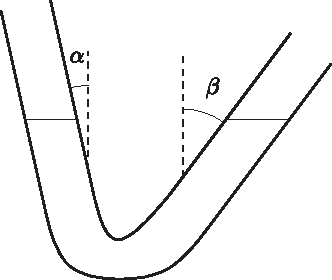
\includegraphics[width=0.5\linewidth]{2008-v3g-08-yl}
\end{center}

\hint
Omavõnkesageduse leidmiseks on harilikult kõige mugavam vaadelda väikest hälvet tasakaaluasendist ning uurida, kuidas süsteem edasi käitub. Ülesande kontekstis võib oletada, et õhuke veekiht ühes toru harus kandub teisele toru poolele. See põhjustab lisarõhu toru teises pooles, mis üritab süsteemi tasakaaluasendisse tagasi viia.

\solu
Oletame, et vesi on tasakaalust hälbinud nii, et veekiht, mille kõrguse projektsioon toru sihis on $\delta x$, on kandunud nurga $\alpha$ all olevast toru poolest teise. Veetaseme kõrguste erinevus toru kahe poole vahel on $\delta h = \delta x (\cos (\alpha ) + \cos (\beta ))$, mis tekitab lisarõhu $\delta P = \rho \delta hg$. Lisarõhk mõjub vedelikule jõuga, mille toru sihiline komponent on
\[
F = \delta P S = \rho \delta x (\cos (\alpha ) + \cos (\beta )) gS.
\]
See valem on sarnane vedrupendli valemiga $F = k\delta x$, kus 
\[
k = \rho (\cos (\alpha ) + \cos (\beta )) gS.
\]
Sellise pendli omavõnkesagedus avaldub kui
\[
f = \frac{1}{2\pi} \sqrt{\frac{k}{m}} = \frac{1}{2\pi} \sqrt{\frac{\rho(\cos(\alpha)+\cos(\beta))gS}{m}}.
\]
Seega võime öelda, et toru pooli painutades väheneb vedeliku võnkumise sagedus
\[
\sqrt{\frac{1}{2}(\cos \alpha + \cos \beta)}
\]
korda.
\probend